\newcommand{\Projekt}{Testat}

\documentclass[a4paper,12pt]{article}
\usepackage[a4paper]{geometry}

\usepackage[utf8]{inputenc}
\usepackage[ngerman]{babel}
\usepackage[T1]{fontenc}
\usepackage{booktabs}
\usepackage{multirow}
\usepackage{graphicx}
\usepackage{tabularx}
\usepackage{longtable}
\usepackage{ragged2e}


\title{\Projekt}
\author{Caner Kara, Dennis Behrendt, Sven Wolf, Tim Sibum, Hannes Scherer,Tim Turowski}
\date{\today}

\begin{document}

\maketitle

\includegraphics[width=18cm]{pictures/cover.png}

\newpage
\section{Änderungshistorie}

\begin{flushleft}
		\begin{longtable}{p{2,5cm}p{2cm}p{3cm}p{8,5cm}c}
        %% Tabellenkopf
            \toprule
            \textbf{Version} & \textbf{Datum} & \textbf{Autor} & \textbf{Änderungen}\\
            \midrule\endfirsthead
            \toprule
            \textbf{Version} & \textbf{Datum} & \textbf{Autor} & \textbf{Änderungen}\\
            \midrule\endhead
        %% Tabelleninhalte
            	Version 1.0 & 23.04.2023 & Tim Turowski & Git-Repository angelegt und Pflichtenheft Tex-Dokument \\ \midrule
				Version 1.1 & 26.04.2023 & Tim Silbum & ERM und UML Diagramm zur Datenstruktur eingefügt \\ \midrule
				Version 1.2 & 26.04.2023 & Hannes Scherer & Frontend Prototypen entwickelt \\ \midrule
				Version 1.3 & 27.04.2023 & Tim Silbum & Sequenzdiagramm, Zustandsdiagramm und GUI Skizze \\ \midrule
 				Version 1.4 & 28.04.2022 & Tim Turowski & Bilder ins Pflichtenheft eingefügt und Tabellen angepasst \\ \midrule
				Version 1.5 & 02.05.2023 & Dennis Behrendt & Bezogen auf das erste Feedback: Inhalte korrigiert und Ausformulierungen angepasst \\ \midrule
				Version 1.6 & 03.05.2023 & Hannes Scherer & Bezogen auf das erste Feedback: Frontend Prototypen angepasst \\ \midrule
				Version 1.7 & 06.05.2023 & Tim Turowski & Nach Problemen beim mergen im Repository: Pflichtenheft ist eigenständiges Dokument \\ \midrule
				Version 1.8 & 07.05.2023 & Tim Turowski & Inhalte der Projektmitglieder eingefügt für morgiges Meeting \\ \midrule
				Version 1.9 & 07.05.2023 & Tim Turowski & Inhaltliche Änderungen nach Zwischenbesprechung \\ \midrule
				Version 1.10 & 14.05.2023 & Tim Turowski & Finale Änderungen für morgiges Kundenmeeting: Inhaltliche Anpassung/Ergänzungen der Projektmitglieder hinzugefügt \\ 
            \bottomrule
    \end{longtable}

\end{flushleft}

\newpage

\tableofcontents

\newpage

\section{Zielbestimmung}

Heutzutage günstig Lego-Sets zu erwerben kann auf mehreren Ebenen ein wohlüberlegtes Unterfangen sein. Welche der Lego-Händler bieten die Sets günstig an? Ist es günstiger sich die Einzelteile des Sets einzeln zu bestellen? Was ist wenn bestimmte Einzelteile nicht mehr verfügbar sind? \newline
Das Ziel des Projekts ist genau diese Fragestellungen, durch die Entwicklung eines Tools zur Ermittlung der günstigsten Anbieter, zu beantworten. Das Tool soll dabei auch in der Lage sein, abzuwägen, ob es günstiger ist, das Set oder Einzelteile zu kaufen und zu kombinieren.

\subsection{Musskriterien}
\begin{enumerate}
\item Es soll eine Datenbank mit Stücklisten und Bauteilen geben
\item Die PDF-Bauanleitungen der Lego-Sets werden mit OCR auslesbar sein
\item Ein Crawler bezieht die Preise der unterschiedlichen Händler zur Laufzeit der Suche
\item  Ein Preisvergleich unter den Händlern, im Bezug auf Kauf eines Sets oder der jeweiligen Einzelteile, findet statt
\item Darstellung des Tools als graphische Oberfläche. (Startseite, Benuterverwaltung, Preisvergleich, Warenkorb)
\item Es soll möglich sein Benutzeraccounts anzulegen und diese zu verwalten
\item Drei feste Händler sollen beim Vergleich berücksichtigt werden
\item Auf nicht verfügbare Einzelteile sollte hinreichend hingewiesen werden.
\item Bei der Ausgabe des Vergleichs soll eine Verlinkung zum Produkt, sowie eine Liste der Bauteile, angezeigt werden.
\end{enumerate}

\subsection{Kannkriterien}
\begin{enumerate}
\item Plattform sollte auch auf Mobilgeräten gut dargestellt sein
\item Mehr Händler sollen implementierbar sein
\end{enumerate}

\subsection{Wunschkriterien}
\begin{enumerate}
\item Die ausgegebene Stückliste wird automatisch auf Wunsch in einen Warenkorb des gewählten Shops umgewandelt
\item Filterfunktion um zum Beispiel Figuren ausfiltern zu können
\item Sticker berücksichtigen
\item Eigens kreierte Bauanleitung sind ebenfalls auslesbar
\item Aktuelle Angebote werden hervorgehobe
\item Dashboard: Statistiken zum Suchverhalten unserer Benutzer / Wie erfolgreich war unser Programm?
\item Einzelteile die besonders selten/teuer sind sollten gesondert aufgelistet werden
\item Die Lieferkosten sollen beim Preisvergleich berücksichtigt werden.
\end{enumerate}

\subsection{Abgrenzungskriterien}
\begin{enumerate}
\item Unser Produkt wird keine Verkaufsplattform haben
\item Keine Bevorzugung von Händlern
\item Wir berücksichtigen nur offizielle Klemmbausteine
\item Website ist nur für deutschsprachige Benutzer
\item Alte Sets (vor 2006 erschienen) ohne Stückliste in der Anleitung werden nicht berücksichtigt
\item Wir berücksichtigen keine Retailpreise
\item Bauanleitungen werden nur von der offiziellen Lego-Webseite gecrawelt
\item Die Entwicklungsumgebung sollte vom Kunden gestellt werden
\end{enumerate}

\section{Produkteinsatz}
 Das Produkt soll Benutzer bei Kaufentscheidung unterstützen, außerdem unterstützt es die Benutzer Sets zu bauen die aus irgendwelchen Gründen nicht mehr verfügbar sind.\newline
Das Tool ist für Lego-Enthusiasten und Sammler gedacht, die nach dem günstigsten Angebot suchen. Das Tool kann auch von Einzelpersonen oder Unternehmen genutzt werden, die große Mengen an Lego-Sets kaufen möchten. \newline
\includegraphics[width=18cm]{pictures/3.UseCase.png} \newpage
\section{Produktfunktionen}

\subsection{Benutzersicht}

/F10/ \newline
Geschäftsprozess: Über eine Suchmaske können Lego Setnummern eingeben werden\newline
Vorbedingung: User befindet auf der Website des LegoGCT\newline
Nachbedingung: Nach der Eingabe wird die Datenbank auf die Existenz des Lego Sets geprüft\newline
Fehlerfall: Die Eingegebene Setnummer stimmt nicht mit einer in der Datenbank vorhanden Setnummer überein. Oder Syntaxfehler führt zur falschen Eingabe\newline
Anwender: Akteur im Kontext der Webapplikation\newline
Beschreibung: Über die Suchfunktion kann der Benutzer eine Setnummer eingeben.\newline\newline
/F20/\newline
Geschäftsprozess: Registrierung auf der Webplattform\newline
Vorbedingung: User befindet auf der Website des LegoGCT und hat den Registrieren Button gedrückt\newline
Nachbedingung: User konnte sich Erfolgreich registrieren lassen sein Benutzer Account wurde in einer Datenbank abgelegt\newline
Fehlerfall: E-Mail ist bereits vergeben, Datenbank ist nicht ansprechbar, Passwortsicherheit zu gering\newline
Anwender: Akteur im Kontext der Webapplikation\newline
Beschreibung: Um die vollen Funktionsumfang der Webapplikation zu nutzen. Muss der Benutzer eine Registrierung durchführen.\newline\newline
/F30/\newline
Geschäftsprozess: Anmeldung auf der Webplattform\newline
Vorbedingung: Benutzer befindet auf der Website des LegoGCT und ist ein Registrierter Nutzer\newline
Nachbedingung: Benutzer konnte sich erfolgreich an Webplattform anmelden\newline
Fehlerfall: Eine Anmeldung war nicht erfolgreich, weil Passwort und Benutzername nicht übereinstimmen oder der Benutzer noch keine Registrierung vorgenommen hat.\newline
Anwender: Akteur im Kontext der Webapplikation\newline
Beschreibung: Um die volle Funktion der Webapplikation nutzen zu können, kann sich der Benutzer an der Webplattform anmelden\newline\newline
/F40/ \newline
Geschäftsprozess: Abmelden von der Webplattform \newline
Vorbedingung: Benutzer ist auf der Webplattform angemeldet.\newline
Nachbedingung: Kunde befindet sich wieder auf der Startseite, ihm wird mitgeteilt, dass er sich abgemeldet hat. \newline
Fehlerfall: Abmeldung schlägt fehl \newline
Anwender: Akteur im Kontext der Webapplikation \newline 
Beschreibung: Eine Abmeldung von der Webplattform sollte ermöglicht werden \newline \newline
/F50/\newline
Geschäftsprozess: Darstellung der Stücklisten\newline
Vorbedingung: Benutzer hat nach einer Setnummer gesucht, welche in der Datenbank vorhanden ist.\newline
Nachbedingung: Benutzer bekommt eine Stückliste mit Einzelteilen angezeigt \newline
Fehlerfall: Stückliste konnte nicht dargestellt werden, da zu viele Einzelteiler bei Händler nicht zur Verfügung stehen. \newline
Anwender: Akteur im Kontext der Webapplikation \newline
Beschreibung: Dem Benutzer wird eine Stückliste des Legosets ausgegeben nach dem der Benutzer gesucht hat. Die Stückliste enthält die Einzelteile mit folgenden Attributen Einzelteilnummer, Anzahl, Preis, URL \newline\newline
/F60/\newline
Geschäftsprozess: Minimieren der Stücklisten\newline
Vorbedingung: Benutzer bekommt eine Stückliste mit Einzelteilen angezeigt\newline
Nachbedingung: Benutzer bekommt nur noch den Endpreis angezeigt\newline
Fehlerfall: keinen\newline
Anwender: Akteur im Kontext der Webapplikation \newline
Beschreibung: Der Benutzer möchte eine übersichtlichere Anzeige haben und minimiert deshalb die Stückliste, um sich den Endpreis übersichtlicher darstellen zu lassen.\newline\newline
/F70/\newline
Geschäftsprozess: Anzeigen der Historie\newline
Vorbedingung: Benutzer sollte auf der Webplattform angemeldet sein\newline
Nachbedingung: Benutzer kann sich seine persönliche Historie anzeigen lassen\newline
Fehlerfall: Benutzer hat bisher noch keinen Suchvorgang gestartet\newline
Anwender: Akteur im Kontext der Webapplikation\newline
Beschreibung: Für Angemeldete Nutzer steht die Historie vergangener Suchen zur Verfügung. Diese unterstützt den Benutzer bereits gesuchte Sets wiederzufinden.\newline\newline
/F80/ \newline
Geschäftsprozess: Historie Suchen erneut durchführen \newline
Vorbedingung: Benutzer ist auf Webplattform angemeldet \newline
Nachbedingung: Kunde bekommt die Stückliste sowie den Endpreis angezeigt.\newline 
Fehlerfall: Einzelteil oder Set nicht mehr verfügbar \newline
Anwender: Akteur im Kontext der Webapplikation \newline
Beschreibung: Um vergangene Suchen erneut aufzurufen, um eventuelle  Preisveränderungen zu dokumentieren. \newline \newline
/F90/ \newline
Geschäftsprozess: Passwort ändern \newline
Vorbedingung: User klickte auf "Passwort ändern" und gab neues Passwort ein \newline
Nachbedingung: Passwort wurde in Datenbank angepasst \newline
Fehlerfall: Passwort das selbe wie zuvor, Passwort hat zu niedrigen Sicherheitsfaktor \newline
Anwender: Akteur im Kontext der Webapplikation \newline
Beschreibung: Der Benutzer möchte sein Passwort ändern \newline \newline
/F100/ \newline
Geschäftsprozess: Email-Adresse ändern \newline
Vorbedingung: User klickte auf "Email-Adresse ändern" und gab neue Email-Adresse ein \newline
Nachbedingung: Email-Adresse wurde in Datenbank angepasst \newline
Fehlerfall: Email-Adresse die selbe wie davor, Eingabe entsprach keiner Email-Adresse \newline
Anwender: Akteur im Kontext der Webapplikation \newline
Beschreibung: Der Benutzer möchte seine Email-Adresse ändern \newline \newline
\newline \newline
\subsection{Produktfunktionen Backend} 

/F110/ \newline
Geschäftsprozess: Nach neuen PDFs/Legosets suchen \newline
Vorbedingung: Festgelegte Dauer ist erreicht worden \newline
Nachbedingung: Neue PDFs/Legosets wurden gefunden oder auch keine neuen PDFs werden gefunden \newline
Fehlerfall: Suche konnte nicht durchgeführt werden \newline
Anwender: Geschäftslogik, Lego.com, Datenbank \newline
Beschreibung: Um die Datenbank auf aktuellen stand zu halten, ist es erforderlich die Datenbank in regelmäßigen abständen zu aktualisieren und mit neuen Datensätzen zu füllen \newline \newline
/F120/ \newline
Geschäftsprozess: Neue PDFs auslesen \newline
Vorbedingungen: Es wurde nach neuen PDFs gesucht \newline
Nachbedingung: Die neuen PDF/s wurde via OCR ausgelesen \newline
Fehlerfall: Das auslesen der PDF/s schlägt fehl \newline
Anwender: Geschäftslogik, Lego.com, Datenbank \newline
Beschreibung: Wenn eine PDF gefunden wurde, die anhand der Lego Setnummer nicht einer anderen Nummer in der Datenbank zuzuordnen ist. Wird in die Datenbank mit aufgenommen \newline \newline
/F130/ \newline
Geschäftsprozess: Ausgelesene PDF-Informationen in Datenbank ablegen \newline
Vorbedingungen: Es wurde nach neuen PDFs gesucht \newline
Nachbedingungen: Die PDF-Informationen wurden in der Datenbank abgelegt \newline
Fehlerfall: Daten werden falsch abgelegt, Daten könnten nicht hinterlegt werden \newline
Anwender: Geschäftslogik, Datenbank \newline
Beschreibung: Die vorher gefundenen Informationen, werden nun in einer Datenbank gespeichert. \newline \newline
/F140/ \newline
Geschäftsprozess: Preise bei Händlern abfragen \newline
Vorbedingungen: Setnummer ist in Datenbank vorhanden \newline
Nachbedingungen: Die Preise wurden bei den Händlern abgerufen \newline
Fehlerfall: Die Preise konnten nicht abgerufen werden \newline
Anwender: Geschäftslogik, Datenbank \newline
Beschreibung: Um den Preisvergleich zu ermöglichen müssen die Preise einzeln bei den Händlern abgefragt werden. \newline \newline
/F150/ \newline
Geschäftsprozess: Einzelteil-Preise berechnen \newline
Vorbedingung: Preise und Stücklisten gesammelt \newline
Nachbedingung: alle Preise berechnet und zwischengespeichert\newline
Fehlerfall: keine \newline
Anwender: Geschäftslogik \newline
Beschreibung: Die zuvor gesammelten Stücklisten und Preise werden zusammengerechnet und für alle, eingebetteten, Shops der Gesamtpreis berechnet. \newline \newline
/F160/ \newline
Geschäftsprozess: Benutzeraccount in Datenbank aufnehmen \newline
Vorbedingung: Der Benutzer gab Benutzername, Email-Adresse und Passwort ein \newline
Nachbedingung: Der Benutzeraccount wurde der Datenbank hinzugefügt \newline
Fehlerfall: Datenbank ist nicht erreichbar \newline
Anwender: Geschäftslogik, Datenbank \newline
Beschreibung: Die Benutzeraccount-Daten werden in der Datenbank verschlüsselt und hinterlegt.
\newline \newline

\section{Produktdaten}
\subsection{Produktdaten}
\includegraphics[width=18cm]{pictures/5.1.System.png}

\subsection{Ergänzungen}
\subsubsection{Benutzerdaten}
Die Persönlichen Daten der Benutzer sollen auf der Datenbank gespeichert werden. Zu den Benutzerdaten gehören: \newline
- Username \newline
- E-Mail-Adresse \newline
- Passwort \newline
- Berechtigungen \newline
- Eine Historie der Sets, welche gesucht worden sind \newline
Die Passwörter der Nutzer werden gehashed auf der Datenbank gespeichert. Dies kann die Speicherung von Sensiblen daten sichern. Der Klarname der Nutzer wird nicht gespeichert, sondern lediglich ein Nutzername. Nutzern wird eine Berechtigung zugewiesen. So können einfache Endanwender lediglich die Funktionen nutzen. Die Administratoren hingegen haben zusätzlich den Zugriff aus einem Dashboard mit Statistiken zu den Suchanfragen.

\subsubsection{Result}
Das Result Objekt beinhaltet alle Informationen, welche bei dem gesamten Prozess zusammengetragen worden sind. Dazu gehört eine Repräsentation des gesuchten Sets und dessen Einzelteile. Zudem verwaltet Result die gefundenen Shop Angebote der Einzelteile des Sets. Das Result Objekt verfügt über eine Funktion die Einzelteile zu Bewerten. Dabei soll ein Wert geliefert werden, welcher den Einzelteilpreis, die Häufigkeit im Set, den Set preis und gegebenenfalls die Verfügbarkeit des Teils einbezieht. Dieser Wert dient als Indikator, ob das Einzelteil besonders ist. Die Metadaten über die Suchanfrage werden auch in Result gespeichert.

\subsubsection{LegoSet}
Ein Lego Set Objekt repräsentiert ein Lego Set und seine Einzelteile. Es Verwaltet auch den aktuellen Wert des Sets und die Verfügbarkeit. Eine URL zum Download der PDF wird auch in diesem Objekt verwaltet. 

\subsubsection{Einzelteilmarktwert}
Die Objekte vom Typ Einzelteilmarktwert sollen zu einem bestimmten Lego Teil jeweils den Entsprechenden Preis eines Bestimmten Anbieters speichern. Zudem verwaltet es die URL zu dem Angebot und den Zeitpunkt der Peis Abfrage. Wenn der Shop eine Bestands Angabe macht, ist auch möglich diese in dem Objekt zu speichern. 

\subsubsection{Bauanleitung}
Bauanleitungen sind PDF-Dateien. Diese PDF-Dateien haben auf den Letzten Seiten eine Stückliste der Einzelteile. Die PDF-Dateien werden nicht gespeichert und nach dem Parsen gelöscht.
\newpage
\section{Anforderungen an Entwicklungsumgebung}
\subsection{Anforderungen}
Bestandsdatenbank soll aufgebaut werden mit Informationen aus den Anleitungen \newline
Die verwendete Datenbank muss in der Lage sein große Datenmengen zu speichern und zu verarbeiten \newline
Preise sollen bei der Suche gecrawlt werden \newline
Der Crawler soll in der Lage sein schnell Preisdaten bei den Anbietern zu crawlen, außerdem soll ein Algorithmus regelmäßig die neuen Anleitungen erkennen und dem Parser übergeben \newline

\subsection{Technische Anforderungen}
6 Core Prozessor \newline
1 TB Speicher \newline
32 GB RAM \newline
Microsoft Windows Server 2019 \newline

\section{Benutzungsoberfläche}
\subsection{Suche}
\includegraphics[width=18cm]{pictures/7.Benutzeroberfläche1.png} 
\subsection{Suchergebnis}
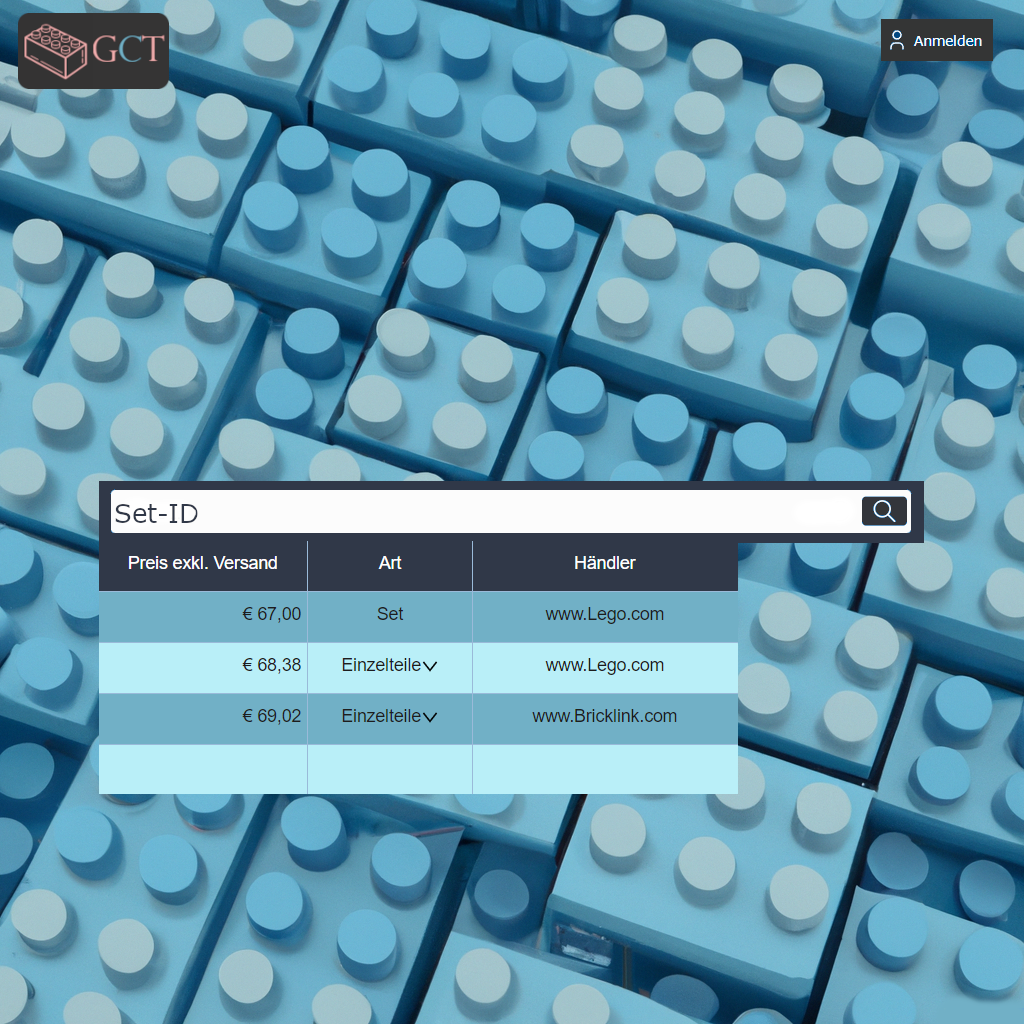
\includegraphics[width=18cm]{pictures/7.Benutzeroberfläche2.png} \newline \newline
\subsection{Registrierungs- und Anmeldefenster}
\includegraphics[width=9cm]{pictures/7.Benutzeroberfläche3.png}
\includegraphics[width=9cm]{pictures/7.Benutzeroberfläche4.png}

\section{Technische Produktumgebung}
\subsection{Produktvorschau}
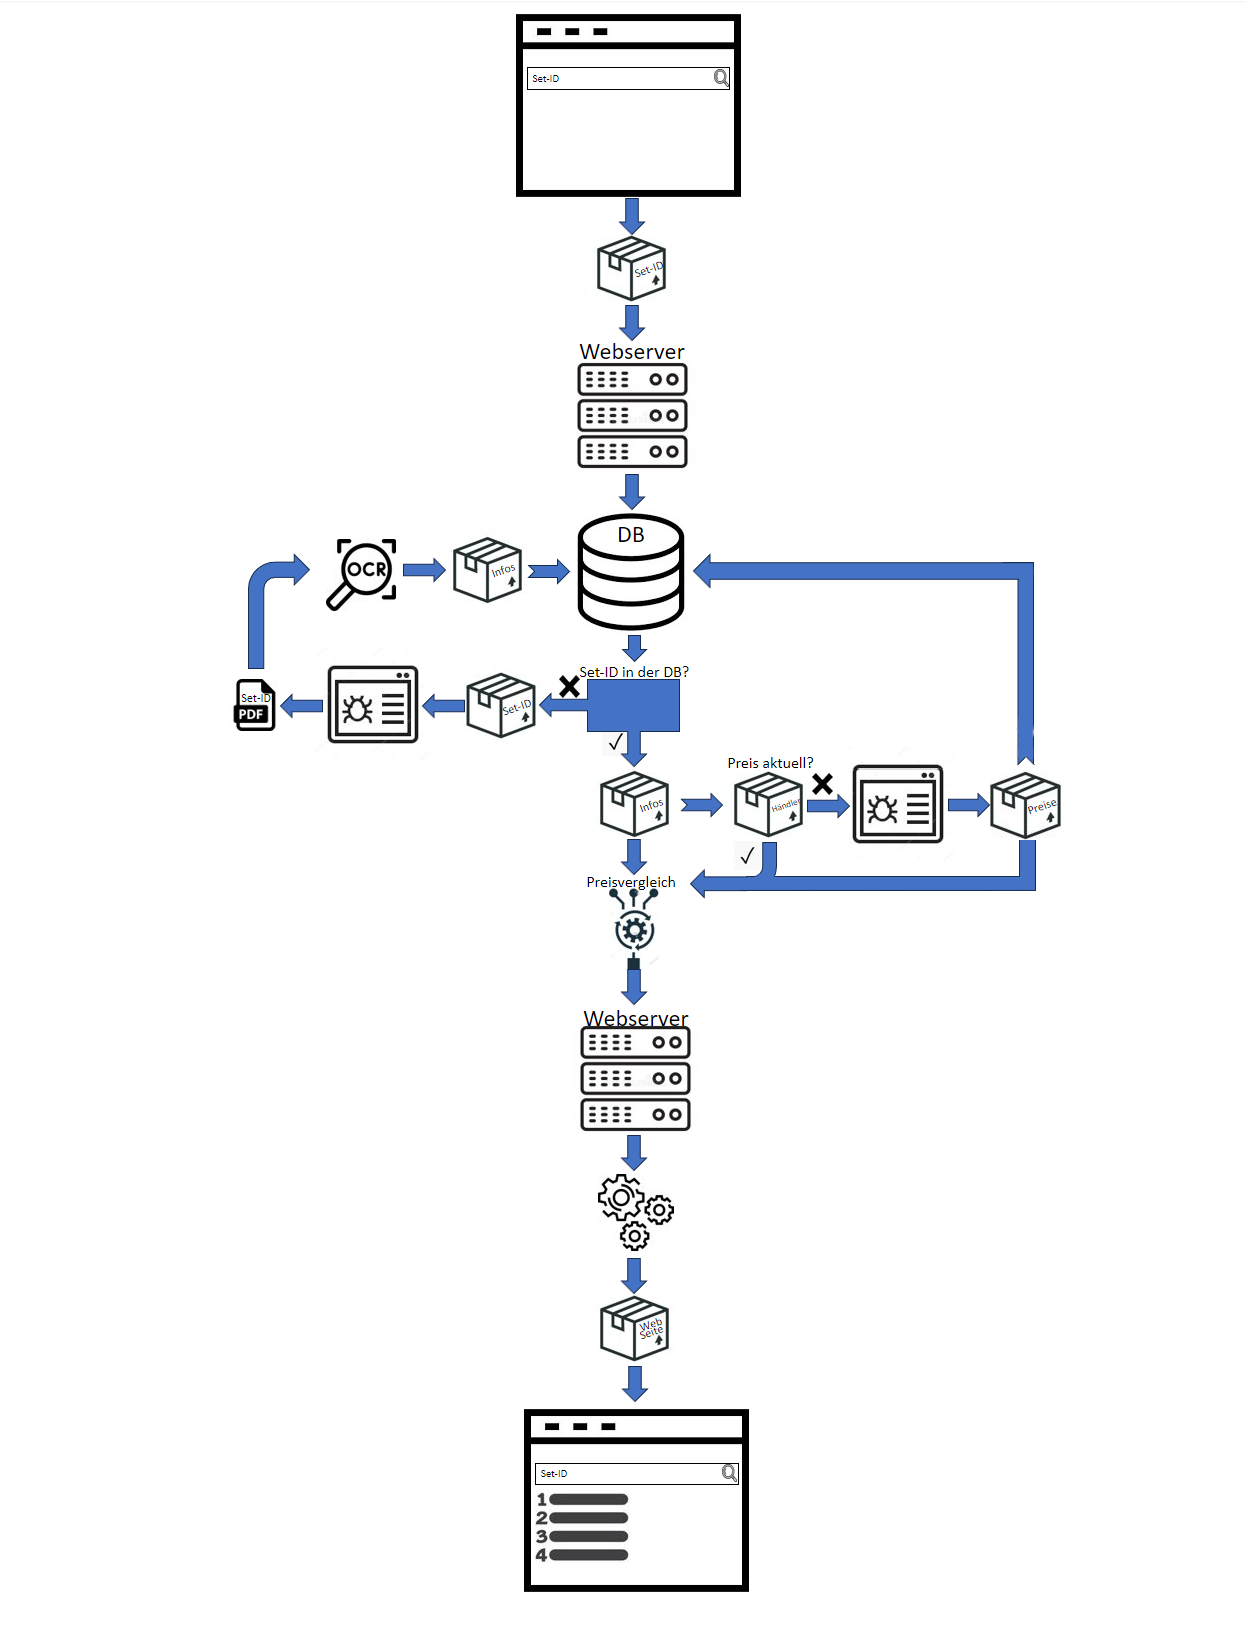
\includegraphics[width=18cm]{pictures/8.TechnischeProduktumgebung.png}

\subsection{Projekt- und Produktumgebungsinformationen}
Git, zur Versionsverwaltung der Dokumentationen und der Software \newline
Tex, zum Dokumentieren \newline
Phython, als Entwicklungssprache für Verwaltung der Daten in DB und Preisvergleich \newline
SQL-Datenbank, zum Speichern der Datensätze \newline
Github, zur Projektplanung \newline
Webserver, zum hosten der Internetseite/Benutzeroberfläche \newline
VM (Server), auf dem die DB läuft, Webserver und Phythonscript ausgeführt wird \newline

\section{Gliederung in Teilprodukte}

\includegraphics[width=18cm]{pictures/9.GliederungDerTeilprodukte.png}
\subsection{Informationen}
\subsubsection{ShopCrawler}
Die Klassen, welche das ShopCrawler Interface implementieren, besitzen die Logik einen Bestimmten Shop zu Crawlen. Für jeden berücksichtigten Shop wird eine Klasse benötigt, welche das Interface ShopCrawler implementiert.  Durch die Verwendung des Interfaces ist es möglich von unterschiedlichen Anbieter Webseiten die gecrawlten Ergebnisse in der gleichen Struktur zurückzugeben.

\subsubsection{TeileFilter}
Der Teile Filter verfügt über Funktionen, welche auf die gecrawlten Daten angewendet werden und prüft, ob die Daten auf die Filtereigenschaften zutreffen.

\subsubsection{AnleitungsCrawler}
Das Interface Shopcrawler liefert eine Struktur eines Parsers für Bauanleitungen. Dadurch ist gewährleistet, dass die Klassen, die das Interface implementieren die geparste Anleitung in der Richtigen Struktur zurückgeben. Die jeweiligen Klassen der Parser müssen zusätzlich eine OCR-Bibliothek einbinden, welche das auslesen von PDF Dateien ermöglicht. 
\newline 
\subsubsection{Anleitungsparser}
Für das Parsen einer Anleitung muss die Anleitung aus dem Internet heruntergeladen werden, dies Ermöglicht der Anleitungsloader. Mit einem Web-Crawler findet er die PDF-Datei zu einer Angegebenen SetID und lädt diese herunter und stellt sie einer Anleitungsparser Implementierung zur Verfügung. 

\subsubsection{Datenzugriffsobjekt}
Das Datenzugriffsobjekt ermöglicht den Zugriff auf die Datenbank. Es besitzt die die nötigen Funktionen die notwendigen Objekte auf der Datenbank zu persistieren oder auf der Datenbank persistente Daten abzurufen. 

\subsubsection{Geschäftslogik}
Teilevergleicher ist die Zentrale Klasse im System.  Die Klasse besitzt die Funktion eine Suche zu starten und sie bündelt alle anderen Objekte im System. Sie bestimmt den logischen Ablauf der Ausführung der Suche.\newpage 
\subsection{Prozess: Anleitungen Parsen}
\includegraphics[width=9cm]{pictures/9.Sequenzdiagramm.png}
\subsection{Prozess: Anleitungen Crawlen}
\includegraphics[width=9cm]{pictures/9.Sequenzdiagramm2.png}
\subsection{Logik: Update der Datenbank}
\includegraphics[width=9cm]{pictures/9.EinspielenNeuerTeile.png} \newpage 

\section{Globale Testfälle}
/T10/ \newline 
Set suchen: Der Nutzer gibt in der Suchleiste die Lego-Setnummer 75355 ein. \newline 
\newline 
/T20/ \newline 
Registrieren: Der Nutzer klickt auf „Registrieren“ und registriert sich mit den Daten: \newline 
-Name: Max Mustermann \newline 
-E-Mail: mustermann@gmx.de \newline 
-Passwort: Passwort1! \newline 
\newline 
/T30/ \newline 
Anmelden: Der Nutzer klickt auf „Anmelden“ und meldet sich mit den in /T20/ benanneten Daten an. \newline 
\newline 
/T40/ \newline 
Abmelden: Der Nutzer Max Mustermann klickt auf „Abmelden“ um sich wieder abzumelden. \newline 
\newline 
/T50/ \newline 
Stückliste anzeigen: Der Nutzer gibt die Lego-Setnummer wie in /T10/ ein. Auf der Ergebnisseite klickt der Nutzer auf „Stückliste anzeigen“, um sich die Einzelteile des Sets anzeigen zu lassen. \newline 
\newline 
/T60/ \newline 
Stückliste minimieren: Der Nutzer agiert wie in /T50/ und klickt darauf auf „Minimieren“,, um die Stückliste wieder einzuklappen. \newline 
\newline 
/T70/ \newline 
Historie anzeigen: Der Nutzer Max Mustermann meldet sich wie in /T30/ an. Er klickt daraufhin auf „Historie“, um sich seine persönliche Such-Historie anzeigen zu lassen. \newline 
\newline 
/T80/ \newline 
In der Historie vergangene Suchen erneut durchführen: Der Nutzer Max Mustermann agiert wie in /T70/. Daraufhin klickt er auf die Setnummer 75355 in der Historie (Link), um die Sucher erneut durchzuführen. \newline 
\newline 
/T90/ \newline Passwort ändern: Der Nutzer Max Mustermann klickt auf „Mein Profil“ und dann auf „Passwort ändern“. Er ändert sein Passwort mit den Daten: \newline 
- Altes Passwort: Passwort1! \newline 
- Neues Passwort: Passwort2! \newline 
- Neues Passwort (Wiederholen): Passwort2! \newline 
\newline 
/T100/ \newline 
Email-Adresse ändern: Der Nutzer Max Mustermann klickt auf „Mein Profil“ und dann auf „Email-Adresse ändern“. Er gibt die Email-Adresse: mustermann2@gmx.de im Textfeld „Neue Email-Adresse“ ein und drückt auf „Speichern“. \newline 
\newline 
/T110/ \newline 
Nach PDF’s der Legosets suchen: Nach einer festgelegten Dauer sucht der PDF Crawler automatisch auf www.lego.com nach PDF’s von Legosets, die noch nicht in der Datenbank liegen. \newline \newline
\newline
/T120/ \newline 
PDF’s der Legosets auslesen: Nachdem ein PDF laut /T110/ gefunden wurde, wird dieses per OCR ausgelesen und gibt die Informationen über die Einzelteile des Sets weiter. \newline 
\newline 
/T130/ \newline 
Ausgelesene PDF-Informationen in Datenbank speichern: Nachdem die Informationen laut /T120/ ausgelesen wurden, werden diese in die Datenbank gespeichert. \newline 
\newline 
/T140/ \newline 
Preise bei Händlern abfragen: Der Nutzer sucht nach dem Lego-Set 13138 (wurde noch nicht gesucht). Der Preis-Crawler bezieht aus den Händlerseiten die jeweiligen Preise der Gesamtsets sowie der Einzelteile des Sets. Diese werden in die Datenbank gespeichert. \newline 
\end{document}